\documentclass[a4paper,12pt]{article}
\frenchspacing
\usepackage[utf8]{inputenc}
\usepackage{a4wide}
%\usepackage[finnish]{babel}
\usepackage[english]{babel}
\usepackage{mathtools}
\usepackage{siunitx}
\usepackage[pdftex]{graphicx}
\usepackage{icomma}
\usepackage{hyperref}
\usepackage{amssymb}
\usepackage{amsmath}
\usepackage{float}
%\usepackage{mhchem}
\usepackage{parskip}
\usepackage{graphicx}
\usepackage{caption}
\usepackage{subcaption}
\usepackage{fancyhdr}
\usepackage{eurosym}
\usepackage{enumerate}
%\usepackage{subfig}
%\usepackage{floatrow}
%\floatsetup[figure]{style=plain,subcapbesideposition=top}
\usepackage{wrapfig, blindtext}


\usepackage[
    backend=bibtex,
    style=numeric,
    sorting=none
  ]{biblatex}
\addbibresource{project.bib}



%%% NEW COMMANDS

\newcommand{\dd}{\,\mathrm{d}}
\newcommand{\exerline}{
\vspace*{.1cm}
\noindent \rule{\textwidth}{1pt}
\vspace*{.1cm}
}

%\usepackage{lastpage}

\pagestyle{fancy}
\fancyhead{}
\fancyhead[LO,RE]{Comp. Phys. -- Project}
%\fancyhead[RO,LE]{Harjoitus 1, 14.9.2012}
\fancyhead[RO,LE]{Kohvakka, 2019}
%\fancyfoot{}
%\fancyfoot[LO,RE]{Kangaslampi / Laaksonen}
%\fancyfoot[RO,LE]{\thepage/\pageref{LastPage}}


\hyphenation{every-where}
\renewcommand{\baselinestretch}{1}

\begin{document}


%\begin{minipage}[t][1.5cm][b]{.2\textwidth}
%\AaltoLogoRandomLarge{0.7}
%\end{minipage}
\begin{minipage}[t][1.5cm][b]{\textwidth}
\begin{center}
\Large{\textbf{Computational Physics}} \\
\vspace*{.1cm}
\Large{\textbf{Project -- 2D FEM Schrödinger solver}}\\
\vspace*{.1cm}
\large{Kassius Kohvakka, 586977}
\end{center}
\end{minipage} 
\vspace{-0.4cm}

\exerline
\vspace{-0.7cm}
\section{Background}

The finite element method (FEM) is a numerical method for solving boundary value problems for partial differential equations used throughout engineering and the sciences. Numerical methods are required in cases where analytical solutions to the problems are intractable to obtain or require abstractions and simplifications which make the solution not applicable in real life. Particularly in engineering, such methods are vital in designing, for instance, load-bearing structures, complicated machine parts, and vehicle chassis which can safely withstand the forces at play and -- if need be -- give in without threatening the lives of the passangers. Problems relating to heat transfer, wave propagation, fluid flow, electromagnetic fields, and other physical phenomena governed by laws expressed in terms of partial differential equations are omnipresent in engineering as well as physics. \cite{rao}

One such problem is solving the time-independent Schrödinger equation. The stationary states of a quantum mechanical system, such as a particle in an external potential, are found by computing the eigenstates of the Hamiltonian operator $\hat{H}$ defined by partial derivatives. While analytic solutions for a few simple potentials are known (e.g. particle-in-a-box and the harmonic oscillator), no analytic solution exists for an arbitrary potential. Thus, numerical computations are required to find approximate solutions in challenging geometries or non-trivial potentials.

The standard approach to the problem is the discretization of the derivatives present in the Hamiltonian, leading to a matrix representation of the Hamiltonian and an eigenproblem for an ordinary matrix. The two common discretization methods, namely, finite difference and FEM, both can be used to this end. The major advantage of the latter over the former is the ability to freely choose the size of the finite elements (triangles in 2D) at each point in the problem domain. This allows significant reductions in the computational cost and memory requirements by using a less dense mesh in regions of lesser importance. Therefore we may take full advantage of the accuracy of the dense grid where it matters while sacrificing less resources for unimportant aspects of the problem \cite{hutton}.

In this project, I implemented a FEM solver for the time-independent Schrödinger equation in two dimensions. The correctness of the solution is assessed by taking a look at the convergence of the energy eigenvalues. Subsequently, the solver is tested for a non-trivial potential. The code was written in python and takes advantage of some of the numerical computation libraries, such as numpy and scipy. The code is visible in a public GitHub repository in \url{https://github.com/kassiuskohvakka/CP-project}.


\cleardoublepage
\section{Theory and methods}

The two-dimensional time-independent Schrödinger equation is given by \cite{griffiths}

\begin{equation}
\label{eq: 2DSchrodinger}
-\frac{\hbar}{2m} \left( \frac{\partial^2 \psi (x,y)}{\partial x^2} + \frac{\partial^2 \psi (x,y)}{\partial y^2} \right) + V(x,y)\psi (x,y) = E \psi (x,y) .
\end{equation}

In order to use FEM to numerically solve Eq. (\ref{eq: 2DSchrodinger}), we expand the wave function $\psi (x,y)$ in a basis of tetrahedral hat functions $\lbrace \phi_i \rbrace_{i=1..N}$ as

\begin{equation}
\label{eq: basisExpansion}
\psi (x,y) \approx \sum_{i=1}^{N} \alpha_i \phi_i(x,y),
\end{equation}

where $N$ is the number of finite elements used in our computation and $\alpha_i$, the coefficients in the linear combination are to be solved for. The linear combination then allows us to construct an approximate solution to the original problem. Setting, for simplicity, $\frac{\hbar}{m} = 1$, writing the partial derivatives more concisely as $\nabla^2 \psi(x,y)$, and substituting our basis expansion in Eq. (\ref{eq: 2DSchrodinger}), we get 


\begin{equation}
\label{eq: schrodingerInFEMBasis}
\left( -\frac{1}{2} \nabla^2 + V(x,y) \right) \sum_{i=1}^{N} \alpha_i \phi_i(x,y)  = E \sum_{i=1}^{N} \alpha_i \phi_i(x,y).
\end{equation}

Rearranging and multiplying both sides by the basis function $\phi_j$, we acquire

\begin{equation}
\sum_{i=1}^{N} \left[ -\frac{1}{2} \phi_j(x,y) \nabla^2 \phi_i(x,y) + \phi_j(x,y) V(x,y) \phi_i(x,y) \right]  \alpha_i   = E \sum_{i=1}^{N} \alpha_i \phi_j(x,y) \phi_i(x,y).
\end{equation}

We can now integrate both sides over the domain $\Omega$ of our problem (and lighten the notation by getting rid of the cluttering $(x, y)$-silliness) to get

\begin{equation}
\label{eq: almostReadyFEMeq}
\sum_{i=1}^{N} \left[ -\frac{1}{2} \left( \int_{\Omega} \phi_j \nabla^2 \phi_i \dd A \right) + \left( \int_{\Omega} \phi_j V \phi_i \dd A \right) \right]  \alpha_i   = \sum_{i=1}^{N} E \left( \int_{\Omega} \phi_j \phi_i \dd A \right) \alpha_i .
\end{equation}

The integrals inside the ordinary parentheses are now matrices. The first of the three still needs to be rewritten by Green's first identity \cite{griffiths2}:

\begin{equation}
\int_{\Omega} \phi_j \nabla^2 \phi_i \dd A = \underbrace{\oint_{\partial\Omega} \phi_j (\nabla \phi_i \cdot \hat{n} )\dd l}_{=0} - \int_{\Omega} \nabla \phi_j \cdot \nabla \phi_i \dd A,
\end{equation}

where the vanishing of the indicated term can be achieved in practice by setting either the basis functions $\lbrace\phi_i\rbrace_i$ or the normal-directional derivatives $\lbrace \nabla \phi_i \cdot \hat{n}\rbrace_i$ at the boundary $\partial \Omega$ to 0 by use of Dirichlet or Neumann boundary conditions, respectively. We can then finally identify the matrices in Eq. (\ref{eq: almostReadyFEMeq}) as the kinetic matrix $T_{ji}$, the potential matrix $V_{ji}$ and the overlap matrix $S_{ji}$:

\begin{equation}
\label{eq: readyFEMeq}
\sum_{i=1}^{N} \left[ \underbrace{\frac{1}{2} \left( \int_{\Omega} \nabla \phi_j \cdot \nabla \phi_i \dd A \right)}_{T_{ji}} + \underbrace{\left( \int_{\Omega} \phi_j V \phi_i \dd A \right)}_{V_{ji}} \right]  \alpha_i   = \sum_{i=1}^{N} E \underbrace{\left( \int_{\Omega} \phi_j \phi_i \dd A \right)}_{S_{ji}} \alpha_i .
\end{equation}

Since the summations on both sides of the equation are just the $j^{\text{th}}$ elements of a matrix-vector product, the elementwise equality implies equality of the resultant vectors and we get

\begin{equation}
\label{eq: matrixFormFEMeq}
(T + V)\alpha = ES\alpha,
\end{equation}

which is a generalized eigenvalue problem involving our known matrices. Solving this, we acquire as eigenvectors the coefficient vectors $\alpha$ approximating the true eigenstates as per the linear combination (\ref{eq: basisExpansion}) and the corresponding approximate energies $E$ of the eigenstates as eigenvalues.





\begin{figure}[H]
\centering
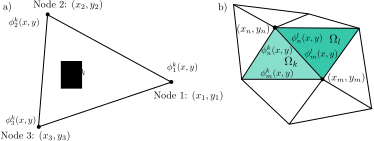
\includegraphics[width=\textwidth]{../figs/triangle.pdf}
\caption{a) A triangular element $\Omega_k$ of the domain together with the three vertices or nodes, each being the center of a FEM basis function $\phi$. Note that at each triangle, only three basis functions are nonzero, and each of them is affine over $\Omega_k$. b) Illustration of the triangulation. The basis functions centered at $(x_n, y_n)$ and $(x_m, y_m)$ overlap only in two triangular elements $\Omega_k$ and $\Omega_l$. Note that in both domains, the functions are affine but not the same as FEM basis functions are piecewise linear.}
\label{fig: triangles}
\end{figure}

The triangulation of the domain $\Omega = [0,1]\times[0,1]$ was done by using \texttt{pygmsh}, a python wrapper for the mesh generator tool Gmsh \cite{PYGMSHdoc}. Having constructed the triangular subdomains $\lbrace \Omega_k \rbrace_k$, construction of the required matrices can be achieved by integrating suitable functions over the subdomains. Integration over an arbitrary triangle can be done by a number of quadratures and was done in practice by utilizing \texttt{quadpy}, a python library for numerical integration. The generalized eigenvalue problem was solved using \texttt{scipy.linalg.eigh}, a library solver for eigenvalue problems involving Hermitian matrices.

The explicit formulas for the piecewise affine hat basis functions for each of the subdomains must be constructed to compute $T$, $V$ and $S$. Over the arbitrary subdomain $\Omega_k$ the relevant basis functions located at the vertices are given by

\begin{eqnarray}
\phi_1^k(x,y) &= \frac{1}{2A_k} \left[ (x_2y_3 - x_3y_2) + (y_2 - y_3)x + (x_3-x_2)y \right] \\
\phi_2^k(x,y) &= \frac{1}{2A_k} \left[ (x_3y_1 - x_1y_3) + (y_3 - y_1)x + (x_1-x_3)y  \right] \\
\phi_3^k(x,y) &= \frac{1}{2A_k} \left[ (x_1y_2 - x_2y_1) + (y_1 - y_2)x + (x_2-x_1)y \right]
\end{eqnarray}

where $A_k$ is the area of the triangle $\Omega_k$ and the labelling of the nodes and basis functions is as in Fig.~\ref{fig: triangles} a). These functions and their simple gradients are easily implemented by some modular arithmetic magic.

After defining a suitable potential function $V(x,y)$, we are ready to start constructing the matrices. Each of the matrices is of size $N \times N$, with row $i$ containing nonzero elements on all columns $j$ if there exists an edge connecting nodes $i$ and $j$, i.e. if the basis functions $\phi_i$ and $\phi_j$ overlap. The value of each of the nonzero elements is the sum of the integral of the relevant functions over the two (or, on the boundary, just one) common triangular subdomains. See Fig.~\ref{fig: triangles} b) and the colored relevant subdomains. Computing the integrals in Eq.~(\ref{eq: readyFEMeq}) and carefully inserting them into the matrices, we are left with all the pieces needed to solve the generalized eigenvalue problem in Eq.~(\ref{eq: matrixFormFEMeq}).

\cleardoublepage

\section{Results}

\subsection{Testing solver and convergence}

\begin{wrapfigure}{r}{0.5\textwidth}
\vspace{-20pt}
\hspace{10pt}
\begin{center}
\includegraphics[width=0.45\textwidth]{../figs/gauss_pot.pdf}
\caption{The potential landscape used in initial tests of the FEM solver. The blue region in the middle is the Gaussian potential minimum and the red region is a high potential barrier approximating an infinite potential well. The blue dots are the triangulation nodes for $N=3436$. }
\label{fig: gaussPot}
\end{center}
\end{wrapfigure}
The initial tests were carried out with simple Gaussian potential minimum in a $[0,1]\times[0,1]$ unit square. The potential landscape is shown in Fig.~\ref{fig: gaussPot} along with the mesh points created by the \texttt{pygmsh} triangulation. The solver was run for this potential and triangulation and the resulting eigenstates and -energies are shown in Fig.~\ref{fig: gaussEigFuncs}. Visual inspection reveals at least that there are no catastrophic errors in the matrices or the solver.

In addition to simple visual inspection, we can also, for instance, check whether the energy eigenvalues got from the solver seem to be converging to a given value as the dimension $N$ of the FEM basis is increased. The apparent convergence of the five lowest energy eigenvalues is shown in Fig.~\ref{fig: gaussEigVals}. At around $N=3500$, the eigenvalues seem to no longer be changing sporadically, implying that our FEM approximation may be getting quite close to the true solution. Given large enough basis dimension, our solver therefore seems to be solving the problem correctly.

The Dirichlet boundary conditions were enforced by removing the rows and columns corresponding to boundary points from the matrices $H$ and $S$ before solving the generalized eigenvalue problem, effectively setting the coefficients of the FEM basis functions centered at nodes on the boundary to zero. In some simulations and with some mesh sizes, this seemed to create stability issues in the solver. To counteract these problems, a high potential barrier was introduced to the boundaries of the problem domain. Approximating the infinite potential barrier normally achieved by simply enforcing the zero boundary condition, this seemed to be enough to stabilize the solutions. 


\begin{figure}[H]
\centering
\vspace{-5cm}
\includegraphics[width=\textwidth]{../figs/eigenfuncs_gauss.pdf}
\caption{The six lowest-energy eigenstates in the Gaussian potential well with $N=3436$. Note that it seems based on our FEM solution that only three of the states are bound to the potential minimum. Notice also the near-degenerate state pairs $(\psi_1, \psi_2)$ and $(\psi_4, \psi_5)$.}
\label{fig: gaussEigFuncs}
\end{figure}



\begin{figure}[H]
\centering
\includegraphics[width=0.7\textwidth]{../figs/energy_convergence.pdf}
\caption{The convergence of the energy eigenvalues as the FEM basis dimension $N$ increases.}
\label{fig: gaussEigVals}
\end{figure}

\subsection{More interesting potential -- less uniform mesh}

To inspect the behaviour of the solver in a different potential landscape, we define a 2D ring-shaped potential well, surrounded on the inside and outside by a high potential. Next, we would like to achieve something like an adaptive meshing scheme to try out our solver with a noticably non-uniform mesh and to keep our FEM basis dimension manageably low while spending our mesh points where it matters, around areas of interesting eigenstate behaviour.

I quickly realized that as it stands, the \texttt{pygmsh} tool kit used in the triangulation lends itself quite poorly to adaptive meshing, so the next best thing was done. The triangulation software was more manually instructed to create smaller finite elements around the ring-shaped potential well, while creating larger triangles both outside and inside the ring. Both the potential landscape and the non-uniformly distributed mesh points created by the modified triangulation algorithm are shown in Fig.~\ref{fig: circlePot}.

\begin{wrapfigure}{l}{0.5\textwidth}
\vspace{-20pt}
\hspace{-30pt}
\begin{center}
\includegraphics[width=0.45\textwidth]{../figs/circle_pot.pdf}
\caption{The ring-shaped potential landscape. The blue (red) color denotes low (high) potential. The blue dots are the triangulation nodes for $N=4763$. Note that the distrubution of the nodes is highly non-uniform. }
\label{fig: circlePot}
\end{center}
\end{wrapfigure}

The modified mesh does little to make solving the generalized eigenproblem any harder. Fig.~\ref{fig: circleEigFuncs} shows the six lowest-energy eigenstates inside the ring-shaped potential well. The eigenstates seem to obey intuition as increase in energy generally translates directly in an addition of a symmetrically-distributed antinode. Interestingly, the more accurate mesh seems to be able to differentiate between the two near-degenerate states $\psi_1$ and $\psi_2$, whose only difference is the orientation of the line connecting the antinodal points. Possibly due to the boundary being so close by and rectangular, the diagonally-oriented antinodes of $\psi_1$ lead to an ever so slightly lower energy in comparison to $\psi_2$ whose antinodes are more oriented along the $x$-axis. Similarly, in eigenstates $\psi_3$ and $\psi_4$ the only difference is the diagonal vs. axial orientation. Here as well the breaking of the symmetry is due to the proximity of the rectangular boundary and should vanish by increasing the simulation box size or by e.g. making the box itself spherically symmetrical.


\section{Conclusions and further studies}
Both the visual inspection of the eigenstates produced by the FEM solver and the apparent convergence of the energy eigenvalues seem to indicate that the solver is working as intended. However, the solver is not terribly efficient especially since all attempts to multithread the construction of the matrices in python seemed only to increase the total running time. This was to be anticipated, however, since python's Global Interpreter Lock~\cite{GILdoc} effectively prevents multicore execution of separate threads. The performance was not completely awful, as solving the ring-shaped potential well problem with $N=4763$ took 76.68 seconds. Increasing the FEM basis dimension further would quickly result in an untracktable running time. With proper parallelization using a suitable (non-interpreted) language, such as C++, the performance could be improved significantly. The vectorization capabilities present in, for instance, the library functions used to integrate over the triangular domains lended themselves poorly to our needs as the integrands differ significantly from domain to domain.




\begin{figure}[H]
\centering
\vspace{-5cm}
\includegraphics[width=\textwidth]{../figs/eigenfuncs_circle.pdf}
\caption{The six lowest-energy eigenstates in the ring-shaped potential well with $N=4763$.}
\label{fig: circleEigFuncs}
\end{figure}

\cleardoublepage

One interesting avenue for further studies would be the implementation of a more automatic adaptive meshing scheme. As stated before, the \texttt{pygmsh} library does not offer ready-made tools for mesh refinement, but programmaticly inserting additional points in the middle of some of the finite element triangles based on e.g. a large value of the laplacian of the eigenstate in the domain might be reasonably straight-forward to implement. The implementation of adaptive meshing would have raised the performance issue in the present code to new heights as the matrix constructions and eigenvalue solutions would have to be redone for each mesh size.

A less manual mesh creation software would also allow for a reasonably achieved increase in the simulation box size. The boundary effects -- not too worrisome even in our tiny simulation domain -- would be further suppressed by having a large domain with a comparatively small region of lower potential. With a larger domain, we could more reliably simulate, say, the electron stucture of a 2D hydrogen atom by introducing a $1/r$-type potential to the system.

\printbibliography



\end{document}
